\documentclass[12pt, a4paper]{report}
\usepackage[T1]{fontenc}
\usepackage[utf8]{inputenc}
\usepackage[english]{babel}
\usepackage{frontespizio}
\usepackage[big]{layaureo}
\usepackage{graphicx}
\usepackage{booktabs}
\usepackage{caption}
\captionsetup{tableposition=top,figureposition=bottom,font=small}
\usepackage{tabularx}
\usepackage{subfig}
\usepackage{color}
\usepackage{colortbl}
\definecolor{Gray}{gray}{0.9}
\usepackage{verbatim}
\usepackage{framed}
\definecolor{shadecolor}{gray}{0.97}
\usepackage{biblatex}

\begin{document}
\chapter*{Project 3}
		
The aim of this project is to build a multiclass image classifier based on convolutional neural networks for the provided dataset (\cite{Lazebnik et al., 2006}). 15 categories are present and already divided into trainset (1500 images, 100 per category) and test set (2985 images).

In the first place we build a CNN which act as a baseline (Section 1). Its performance are then compared with the results of some improved CNNs (Section 2) and other classifiers based on pretrained CNNs (Section 3).
	
	
\section*{1. Baseline}
\subsection*{Problem statement}

To begin we built a CNN which act as baseline following the given instructions.	

\subsection*{Approach}

First of all we  defined the structurs needed to feed the network with our data.\\
Specifically we built a new Dataset class which, every time an image is accessed, loads the image itself in memory and applies a given transformation to it.\\
Then, we splitted the training dataset into train and validation and we construcetd two dataloaders which, at each epoch, take care of dividing data in batches and give them to the network. The same approach is also used for test data.

After having defined the needed structures we built a convolutional neural network following the requests, we trained it and finally tested it.
	
\subsection*{Implementation choices}

In order to obtain images having size 64x64, we defined a transformation, consisting in an anisotropic rescaling, to apply to each image when loaded.

Then, to build the training and the validation dataloaders, we split the given dataset in two parts. The validation dataloader access to the 15\% of the images, equally distributed among the classes, and load them all at once. The traning dataloader access the remaining 85\% of the data, which are loaded in batches of size 32, as required.

After that we've built the network following the given architecture which is reported in Table \ref{tab:baseline}. Since we've used cross entropy as loss function, and in python this loss already performs softmax, the corresponding layer is not present in the network. Hence the outputs of the network are scores and not probabilities.
	
\begin{table}[h!]
	\centering
	\caption{Structure of the baseline CNN}
	\begin{tabular}{lll}
		\# & Type & Size \\
		\midrule
		1 & Image Input & 64x64x1 images \\
		2 & Convolution & 8 3x3 convolutions with stride 1 \\
		3 & ReLu & \\
		4 & Max Pooling & 2x2 max pooling with stride 2 \\
		5 & Convolution & 16 3x3 convolutions with stride 1 \\
		6 & ReLu & \\
		7 & Max Pooling & 2x2 max pooling with stride 2 \\
		8 & Convolution & 32 3x3 convolutions with stride 1 \\
		9 & ReLu & \\
		10 & Fully Connected & 15 \\
		11 & Softmax & softmax \\
		12 & Classification Output & crossentropyex \\
		\bottomrule
		\label{tab:baseline}
	\end{tabular}
\end{table}
		
As optimizer we've employed the stochastic gradient descent with learning rate 0.01, momentum 0.9, as set by default.
	
The weights of each layer have been initialized with a gaussian distribution with mean 0 and standard deviation 0.01. The bias of each layer has been set to 0.

By setting the parameters in this way, we were not able to reach a test accuracy of around 30\%. Indeed our network performed as a random classifier, having a test accuracy of less then 7\%. In particular the specified weights were too high for the last two layers using the default learning rate. To reach a statisfactory accuracy, using the required weight initialization, a smaller learning rate was necessary, so we set it to 0.001.

We employed, as a stopping criterion, the early stopping based on the validation loss which is a measure of the generalization error of our classifier. We've made this choice because, even if we may not reach the global minimum of the validation loss, we can train for fewer epochs stopping when the validation loss significantly increase.\\
In our specific implementation we evaluate the validation loss every 5 iterations. At each iteration we compare the validation loss with the best one obtained up to that moment. If the current loss is at least 1\% higher then the saved one, we increase a counter. On the other hand, if the current loss is lower then the saved one we update it, save the parameters of the network and set the counter to zero. We stop the training when a certain number of epochs are performed or when the counter reach the value of the patience. In our case we have decided to perform at most $30$ epochs and set the patience to $20$.
	
\subsection*{Results}

We performed the training as specified above and plot the evolution of the accuracy and of the loss on both training and validation data (Figure \ref{fig:baseline}).

\begin{figure}[h!]
	\centering
	{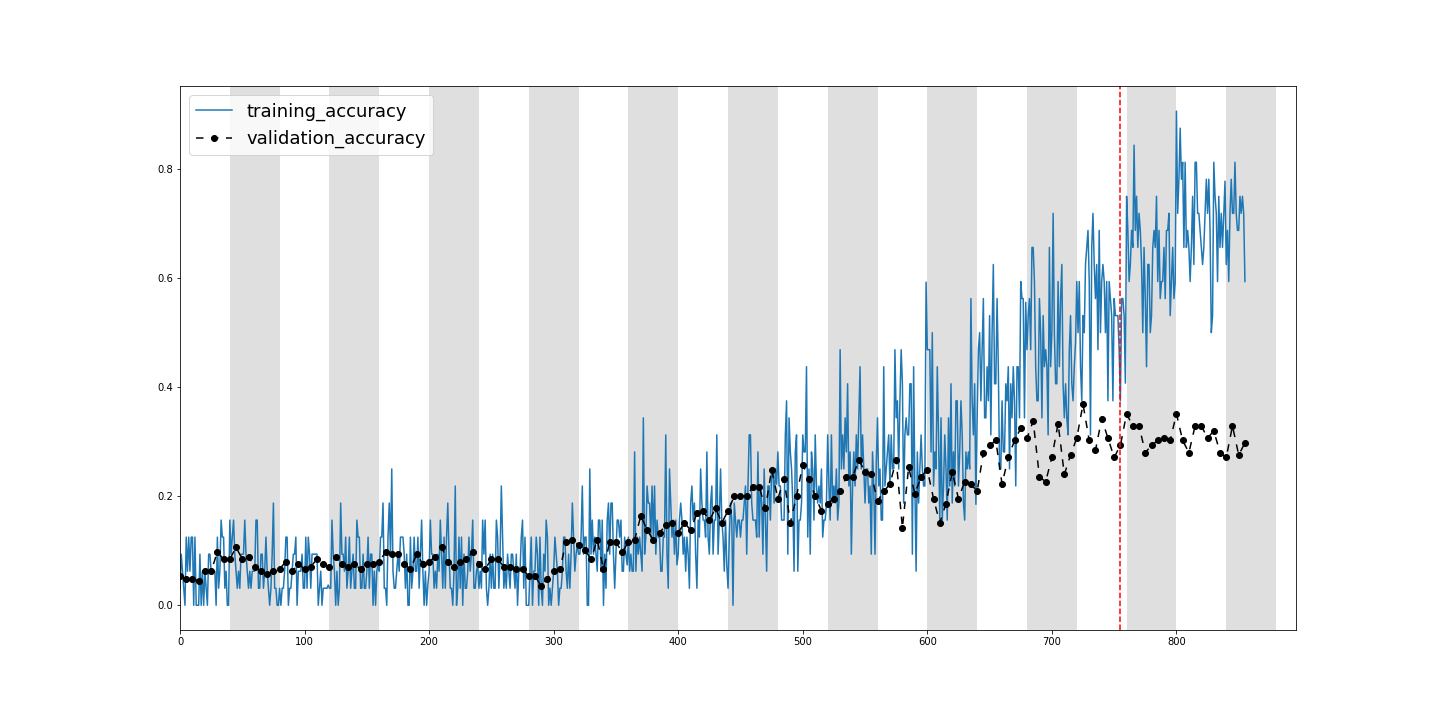
\includegraphics[width=.49\textwidth]{img/baselineAcc}}
	{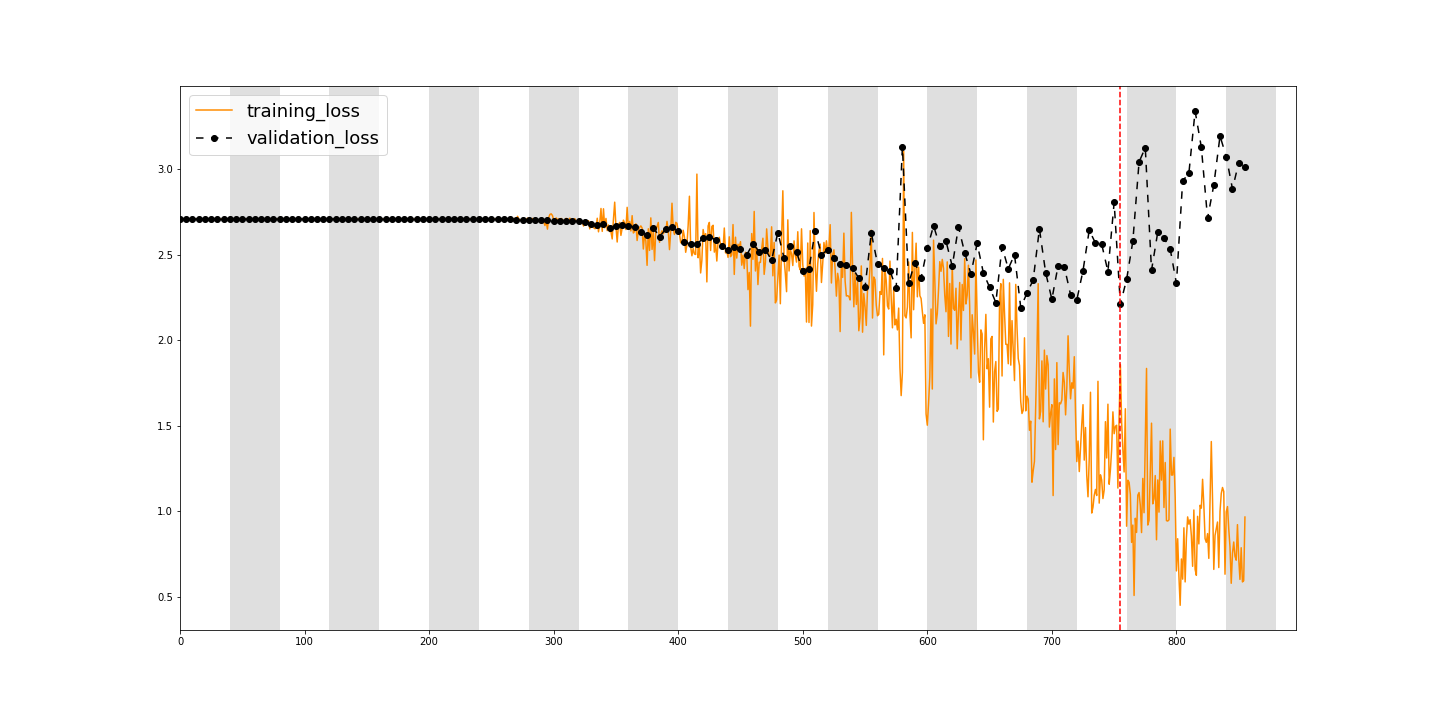
\includegraphics[width=.49\textwidth]{img/baselineLoss}}
	\caption{Training and validation accuracy and loss of the baseline}
	\label{fig:baseline}
\end{figure}

As we can see the training accuracy tends to increase linearly reaching the value of 0.6 before the stop of the training. Looking at the the validation accuracy we notice that, during the first epochs, it takes values similar to the ones of the training accuracy, but after $400$ iterations it begins to be a bit lower then the training metric, stabilizing around values of 0.3.\\
In the same way we can see that the training loss descreases reaching a minimum of around $1.5$. On the other hand the validation loss decreases very slowly and, after $14$ epochs it begins to increase. Hence the training stopped.

We tested the network on the test set obtaining an accuracy of around 31\%. But we've observed a lot of variability in this result: we get values in between 26-32\%. 

\begin{figure}[h!]
	\centering
	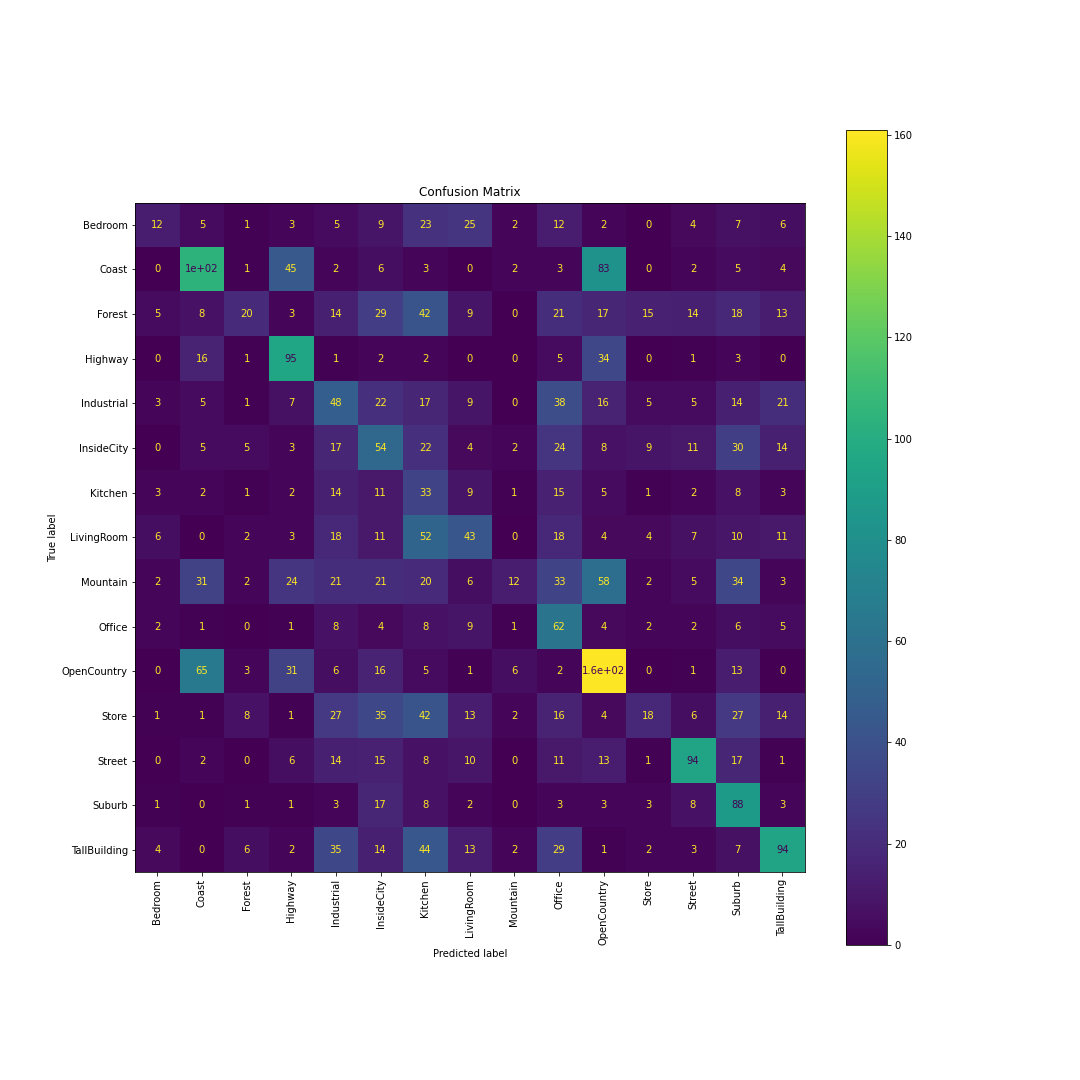
\includegraphics[width=0.9\textwidth]{img/baselineConf}
	\caption{Confusion matrix of the baseline}
	\label{fig:baselinecmatrix}
\end{figure}

Looking at the confusion matrix (Figure \ref{fig:baselinecmatrix}) we notice that there are some misclassifications.

\section*{2. CNN improvements}

\subsection*{Problem statement}
After having developed a CNN which acts as a baseline, we tried to improve the obtained results. In order to do so we applied some transformation to the training data, added some layers and changed some optimizaion parameters. After having found the optimal network we have also build an ensemble of networks.

\subsection*{2.1 Data augmentation}

First of all we perform data augmentation. Since the training set is quite small and only contains $1500$ images, applying some random transformations on the original data set allows to increase the diversity of the training set itself. In this specific case we applied a horizontal flip to each image in the training set only, while the validation and the test sets remained the same.

We tried two different approach. Firstly we defined a new transformation performing a random horizontal flip with probability $0.5$ and we passed it to the trainloader. In this way the transformation is applied with probability $0.5$ to each image every time it is accessed. Hence at each epoch the images are augmented but their number does not increase. Neverthelss we didn't obtain the expected results. Therefore we tried another approach which is to say we actually doubeled the training set. 

We defined a new transformation always performing the horizontal flip. During the training we applied this transformation to each batch and concatenate the transformed batch to the original one. In this way the dimension of each batch double because half of it are the original images and the other half the flipped ones.

We perform the training keeping the options as for the baseline and we obtain the following results (Figure \ref{fig:augmented}).

\begin{figure}[h!]
	\centering
	{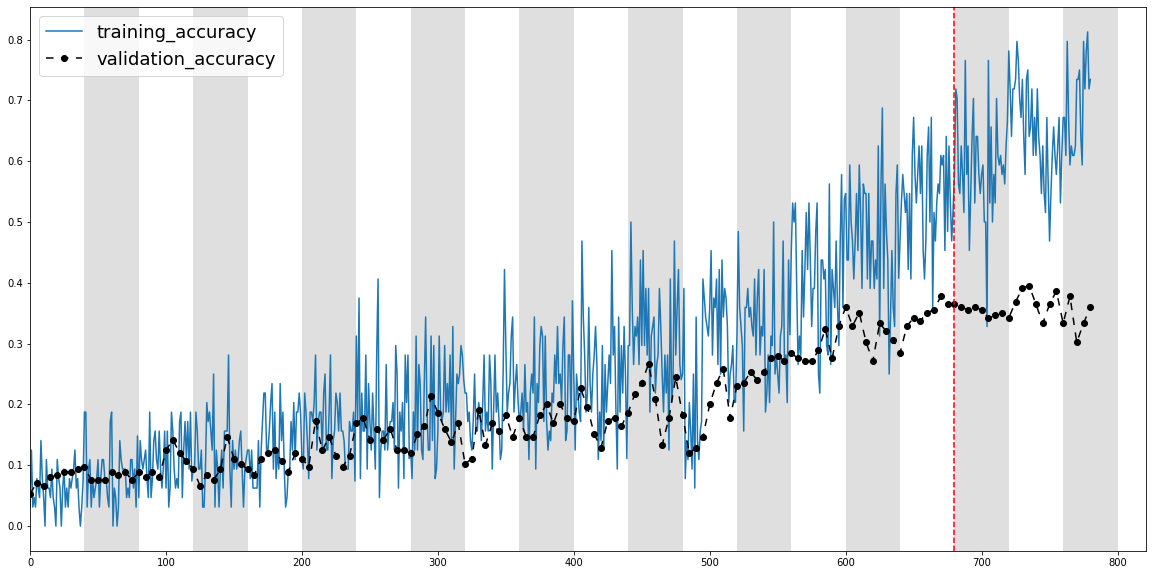
\includegraphics[width=.49\textwidth]{img/aug_accuracy}}
	{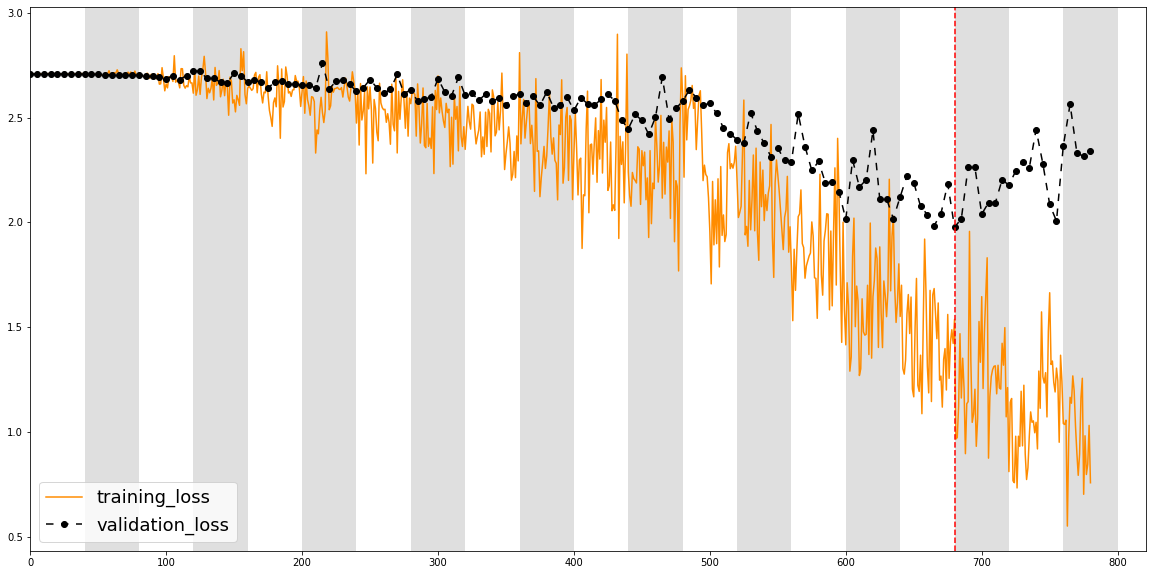
\includegraphics[width=.49\textwidth]{img/aug_loss}}
	\caption{Training and validation accuracy and loss of the basline with data augmentation}
	\label{fig:augmented}
\end{figure}

We can see that the trend of the metrics is similar to the previous one. Neverthelss all of them seems to perform better. In fact both the training and the validation accuracy are slightly higher then in the baseline whereas the training and the validation loss are a bit lower. 

We test our network on the test set and, as expected, we obtained better results.\\
The test accuracy of this network is around 37\%, which is to say almost 7-8\% better then the baseline.

\begin{figure}[h!]
	\centering
	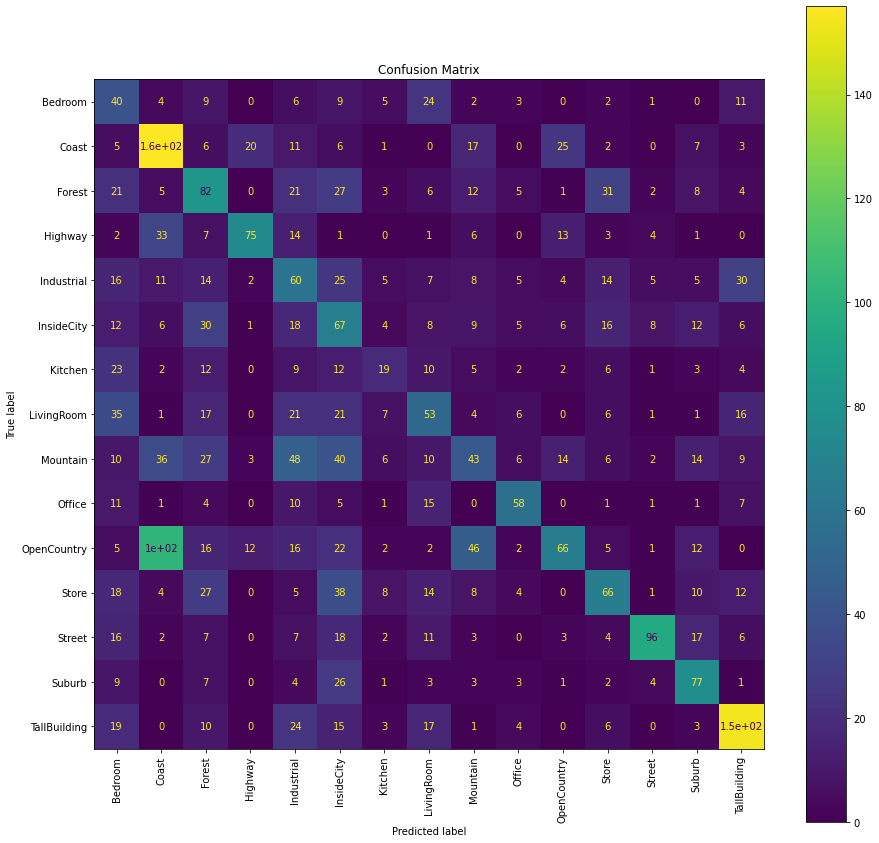
\includegraphics[width=0.9\textwidth]{img/aug_cmatrix}
	\caption{Confusion matrix of the baseline with data augmentation}
	\label{fig:augcmatrix}
\end{figure}

Looking at the confusion matrix (Figure \ref{fig:augcmatrix}) we can see that there are still some misclassifiactions. Expecially the network classifies the 'Open County' as 'Coast' quite often. Nevertheless they are both natural environments, so the error is quite understandable, evan a human being could get them wrong.

\subsection*{2.2 Other improvements}

\subsubsection*{Description of the approach}

After having performed data augmentation we added other layers to the network and changed the optimization parameters in order to obtain better results.

First of all we added a Batch Normalization layer before each reLu layer. In this way the following transformation is applied to the output of the preceding layer:
$$ y = \frac{x - E[x]}{\sqrt{VAR[x]}} * \gamma + \beta$$
The mean $E[x]$ and the standard-deviation $\sqrt{VAR[x]}$ are calculated over the mini-batches and their estimations are then employed during the evaluation phase to normalize the input images. The two parameters $\gamma$ and $\beta$ are vectors of size equal to the input size learned during the training. Thanks to the addition of this layer we avoid divergence of the optimizer due to large changes in the input distribution to each layer. It also reduce dependence on the initialization and acts as a regularizer.

We also add a dropout layer before the fully connected one. In this way, during the training phase, some of the outputs of the layer before are randomly set to zero with a given probability. This technique has proven to be effective for regularization and helps in avoiding overfitting.

Then we changed the size of the convolutional filters increasing their support, going from intput to output, to 3x3, 5x5 and 7x7. In order to obtain an output image of the same size of the input one, we added some replicate padding around the image itself. Specifically we set one padding in the first convolutional layer, two in the second and three in the third. In this way the image do not change size going through the network.

Finally we changed some of the optimization parameters.\\
As first thing we introduced weight normalization. Large values of the network weights can lead to unstable performances and can be an indicator of overfitting of the training data set. To avoid this problem we introduced a regularization term in the objective function which force the network to keep the weight small. In this way the objective function to minimize becomes
$$J(w) = \frac 1 N \sum_{i=1}^n L(f(x_i, w), y_i) + \lambda R(w)$$\\
In addition we tried to modify the value of the learning rate. Increasing its the value to $0.01$ leads the network to not converge to the minimum because the steps are too big. On the other hand, setting it to smaller values, such as $0.0001$, brings to very slow convergence. Hence, since we would like to have a bigger value of the learning rate at the beginning of the training in order to move closer to the minimum, and, after some iterations, a smaller value in order to reach the minimum itself, we introduced a learning rate scheduler. The scheduler decays the learning rate by a given factor every $n$ epochs.\\
After that we modified the batch size setting it to $64$ in order to speed up the computations and obtain a better estimation of the gradient.\\
As last imporovement we changed the used optimizer switching to Adam optimizer, which is faster than the Stochastic Gradient Descent but is still able to obtain the same performances.

\subsubsection*{Implementation choices}

After having introduced the abouve mentioned additional layers, our improved network had the structure reported in the Table \ref{tab:final}.

\begin{table}[h!]
	\centering
	\caption{Structure of the final CNN}
	\begin{tabular}{lll}
		\# & Type & Size \\
		\midrule
		1 & Image Input & 64x64x1 images \\
		2 & Convolution & 8 3x3 convolutions with stride 1 and padding replicate 1 \\
		3 & Batch Normalization & 8 \\
		4 & ReLu & \\
		5 & Max Pooling & 2x2 max pooling with stride 2 \\
		6 & Convolution & 16 5x5 convolutions with stride 1 and padding replcate 2 \\
		7 & Batch Normalization & 16 \\
		8 & ReLu & \\
		9 & Max Pooling & 2x2 max pooling with stride 2 \\
		10 & Convolution & 32 7x7 convolutions with stride 1 and padding replicate 3 \\
		11 & Batch Normalization & 32 \\
		9 & ReLu & \\
		10 & Dropout & p = 0.25 \\
		11 & Fully Connected & 15 \\
		12 & Softmax & softmax \\
		13 & Classification Output & crossentropyex \\
		\bottomrule
		\label{tab:final}
	\end{tabular}
\end{table}

The objective function we aim to minimize was 
$$J(w) = \frac 1 N \sum_{i=1}^n L(f(x_i, w), y_i) + \lambda R(w)$$\\
where $L(f(x_i, w), y_i)$ is the Cross-entropy loss function and the regularization term $R(w)$ is the $L_2$ penalty. We set the $\lambda$ parameter to $0.02$.\\
Concerning the oprimization parameters we set the initial learning rate to $0.001$ and, through the scheduler, it was multiplied by a factor equal to $0.7$ every $3$ epochs. As already said we used Adam as optimizer.\\

\subsubsection*{Results}

We trained the network using the early stopping and setting the patience to $10$ evaluations. we ran the training and plot the evolution of the accuracy and of the loss (Figure \ref{fig:improved}).

\begin{figure}[h!]
	\centering
	{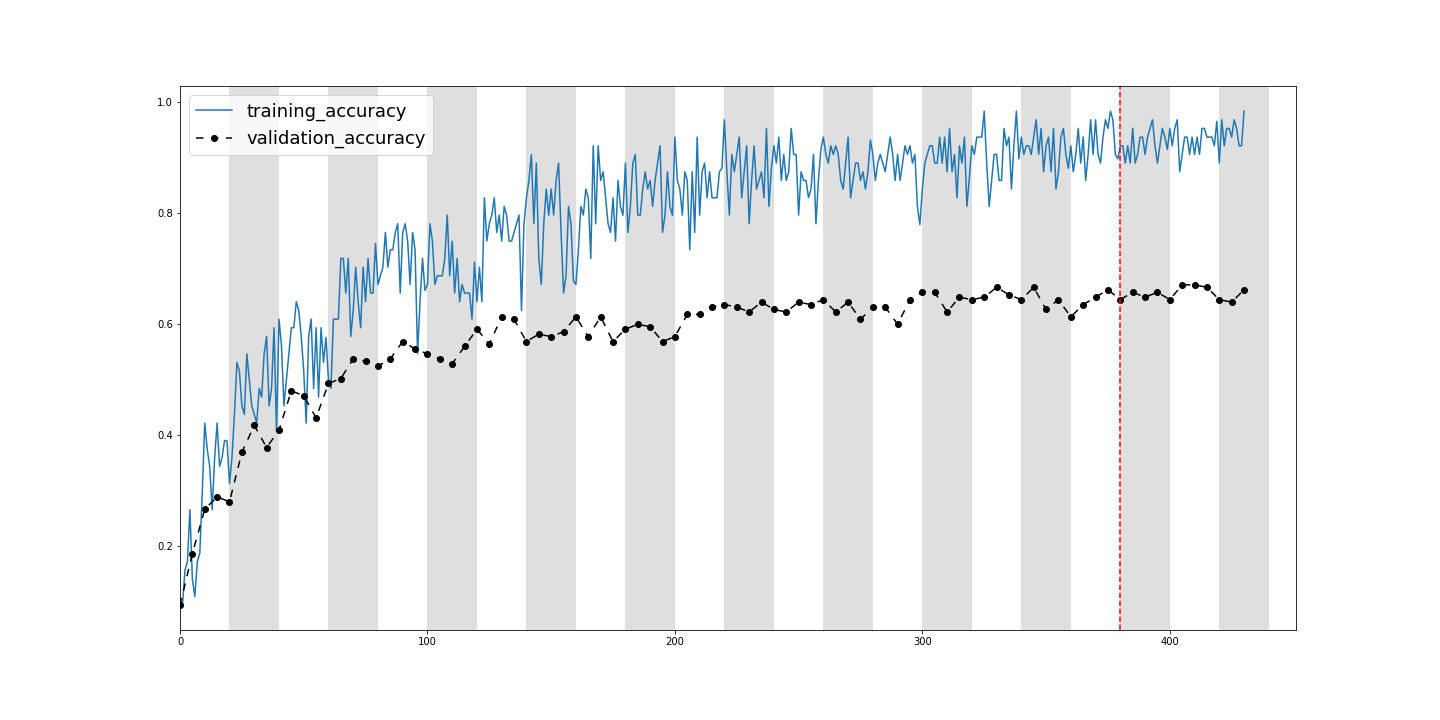
\includegraphics[width=.49\textwidth]{img/final_accuracy}}
	{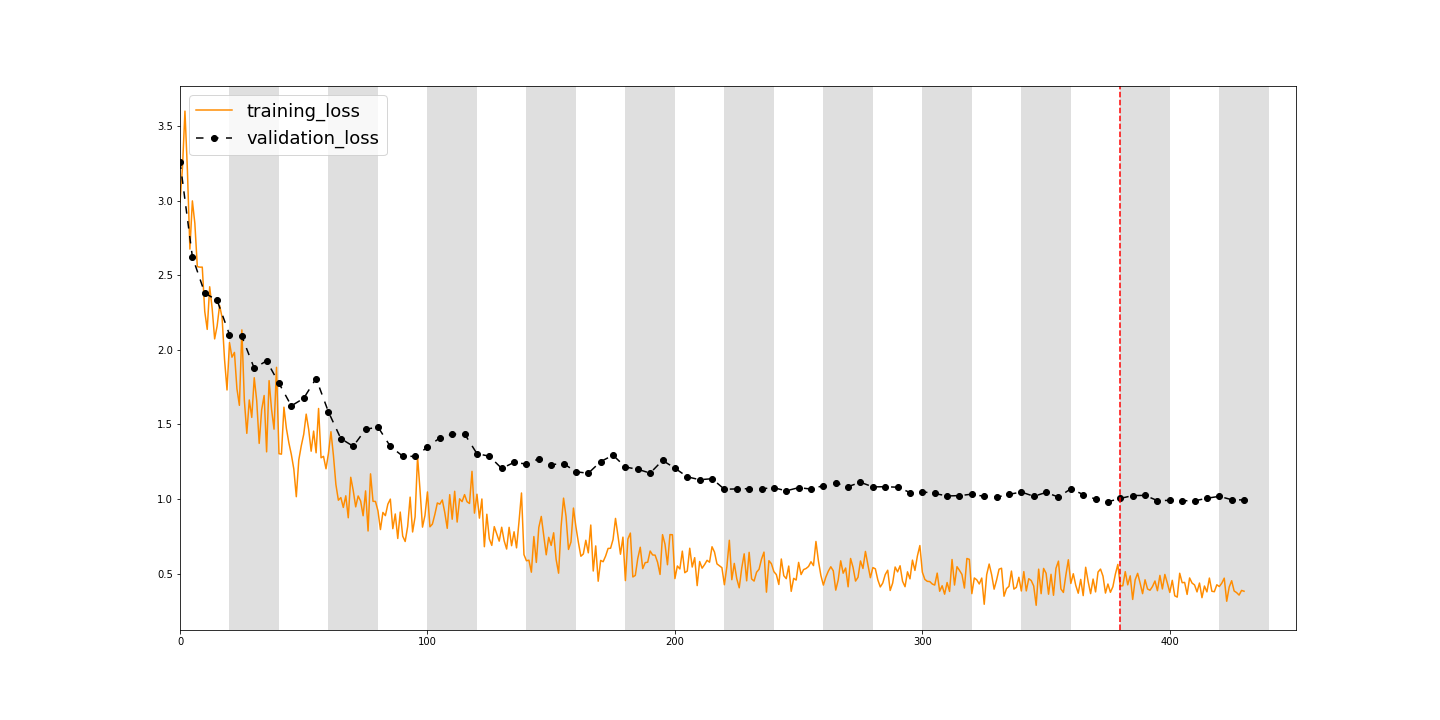
\includegraphics[width=.49\textwidth]{img/final_loss}}
	\caption{Training and validation accuracy and loss of the improved network}
	\label{fig:improved}
\end{figure}

As we can see both the accuracyes and the losses respectivelly increase and decrease much faster then before. Indeed the training accuracy tends to one, while the validation accuracy is stabilized around the value $0.6$. In a similar way the training loss tends to zero, while the vaidation loss is stabilized around $1$. We also noticed that the training stopped because the maximum number of epochs was reached. Therefore we accomplished to reduce overfitting since the validation loss does not increase significalnty even after $30$ epochs.

We test the trained network on the test set and we obtained satisfactory results. Indeed we get a test accuracy of around 65\%.

\begin{figure}[h!]
	\centering
	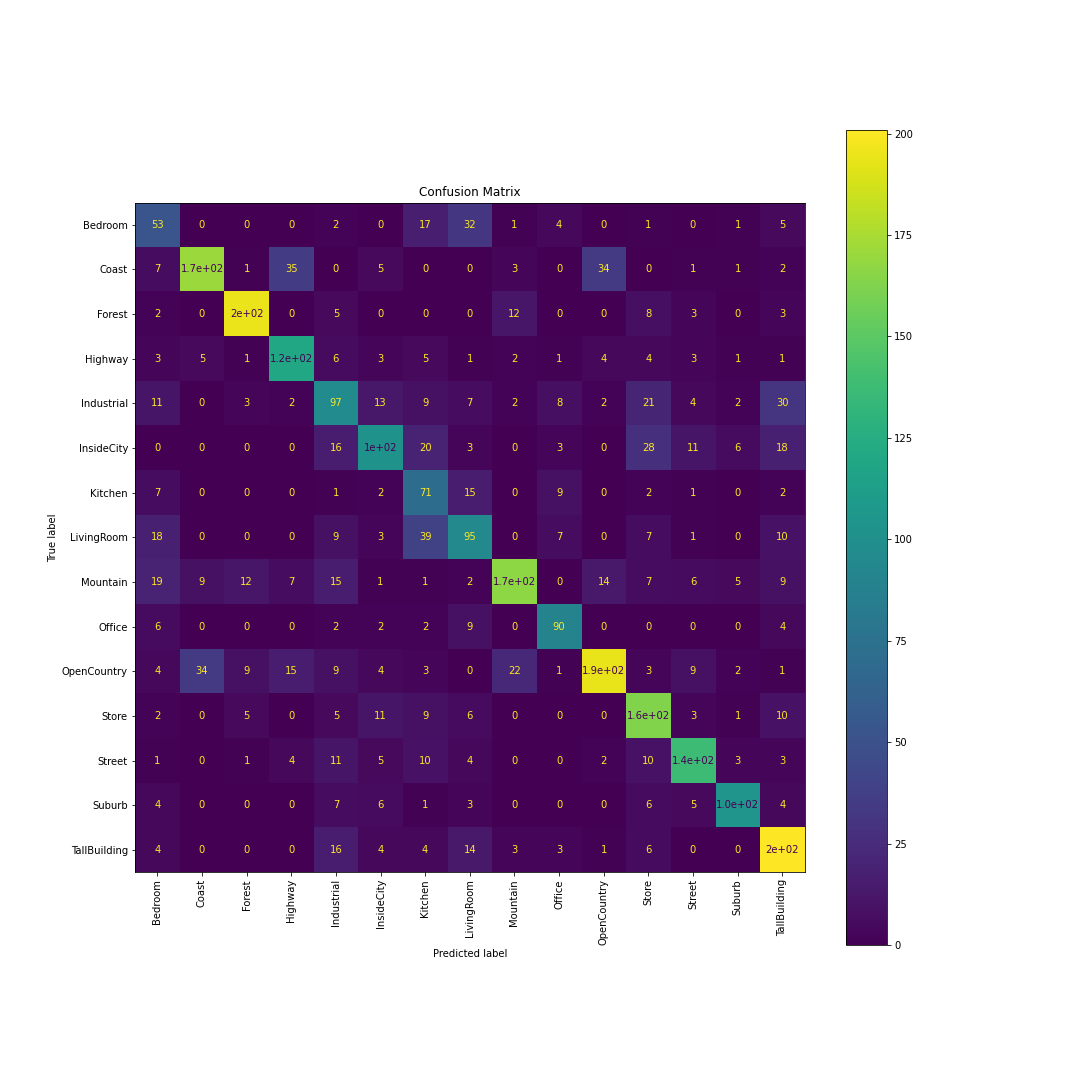
\includegraphics[width=0.9\textwidth]{img/final_cmatrix}
	\caption{Confusion matrix of the improved network}
	\label{fig:improvedcmatrix}
\end{figure}

The confusion matrix (Figure \ref{fig:improvedcmatrix}) confirms the good performances of the network. Even if we still notice some misclassifications expecially among Livingroom and Kitchen and few other classes we are quite satisfied with the obtained result.

\subsection*{Ensemble of networks}

Our improved convolutional neural network performed good enough but its results were quite unstable varying between 62\% and 67\% of test accuracy. Hence, in order to reduce the dependence of the CNN on the training data and on the initialization of the weights, and so reduce the variance of the predictions, we build an esemble of networks, which is to say we build and train several models and combine their predictions together.

We initialized five instances of neural network having the structure specified above and trained them independently. After the training phase we test each network on the test set. We apply each network to each image and make a softmax transformation in order to convert the output scores into probabilities. At this point we calculate the average probability of each class computing the arithmetic mean of the output probabilities of the networks. Finally we predict the class having the higher average probability.

Combining the results of independent networks slightly increase our perormances obtaining a of test accuracy of around 68\%. Nevertheless the main achievements obtainied in this way was the reduced variability of the results. 

\section*{3. Transfer learning}
\subsection*{3.1 Fine tuning}
\subsubsection*{Problem statement}
Build a multiclass classifier for our classification problem fine tuning a pretrained convolutional neural network.

\subsubsection*{Approach}
Take all layers of the chosen pretrained neural network except the last fully connected layer which will be substituted with a new one having suitable output size. Learn only the weights of this last layer freezing all the others. Evaluate the performance of the trained classifier on the test set using the same testing functions as in section 1.

\subsubsection*{Implementation choices:}
We choose to use Alexnet, a convolutional neural network trained on the ImageNet dataset (1.2 million high-resolution images belonging to 1000 categories). 
In the following table we can see the architecture of pretrained Alexnet available on pytorch:

% alexnet architecture 
\begin{table}[h!]
	\centering
	\begin{tabular}{lll}
		\# & Type & Size \\
		\midrule
		Features & & \\
		1 & Image Input & 224x224x3 images \\
		2 & Convolution & 64 11x11 convolutions with stride 4 \\
		3 & ReLu & \\
		4 & Max Pooling & 3x3 max pooling with stride 2 \\
		5 & Convolution & 192 5x5 convolutions with stride 1 \\
		6 & ReLu & \\
		7 & Max Pooling & 3x3 max pooling with stride 2 \\
		8 & Convolution & 384 3x3 convolutions with stride 1 \\
		9 & ReLu & \\
		10 & Convolution & 256 3x3 convolutions with stride 1 \\
		11 & ReLu & \\
		12 & Max Pooling & 3x3 max pooling with stride 2 \\
		\midrule
		Avgpool & & \\
		1 & Avg Pooling & output size 6X6\\
		\midrule
		Classifier & & \\
		1 & Dropout & probability 0.5 \\
		2 & Fully connected & 4096 \\
		3 & ReLu & \\
		4 & Dropout & probability 0.5 \\
		5 & Fully connected & 4096 \\
		6 & ReLu & \\
		7 & Fully connected & 1000 \\
		\bottomrule
		\label{tab:baseline}
	\end{tabular}
\end{table}

It's composed by 5 convolutional layers and 3 fully connected layers. All these trainable layers except for the last fully connected one are followed by ReLu activation function. Moreover there are also 3 maxpooling layers and an adaptive average pooling layer, which calculates the right size of its kernel to obtain the specified output size.

In order to enter this network images need to be preprocessed in the same way the training images have been preprocessed. These are the required transformations:
\begin{itemize}
	\item the network expects each image to be composed by 3 channels so I use PIL library tools to convert image to RGB (it simply replicates the image 3 times).
	\item each channel is normalized with vector of means $[0.485, 0.456, 0.406]$ and vector of standard deviations $[0.229, 0.224, 0.225]$.
	\item resize each image to $[224,224,3]$ performing anisotropic rescaling
\end{itemize}

In order to perform image preprocessing we use the dataloaders used in section 1, we only need to change the transformation to be applied when images are loaded.

We substitute the last fully connected layer having output size 1000 with one having output size 15, the number of our classes. In order to train only the last layer we need to pass to the optimizer only the parameters to be learned: weights and bias of this last layer. Then training and test phases are carried on as in section 1, we are still using cross-entropy loss and stochastic gradient descent with momuntum (learning rate 0.001 and momentum 0.9).
Also in this case we initialize the weights using a gaussian distribution with mean 0 and standard deviation 0.01.

\subsubsection*{Results}

We use again early stopping based on validation loss to avoid overfitting and reduce the computational cost, setting the patience parameter to 20. Loss and accuracy on training and validation sets are reported (Figure \ref{fig:finetune}).

% two training plots
\begin{figure}[h!]
	\centering
	{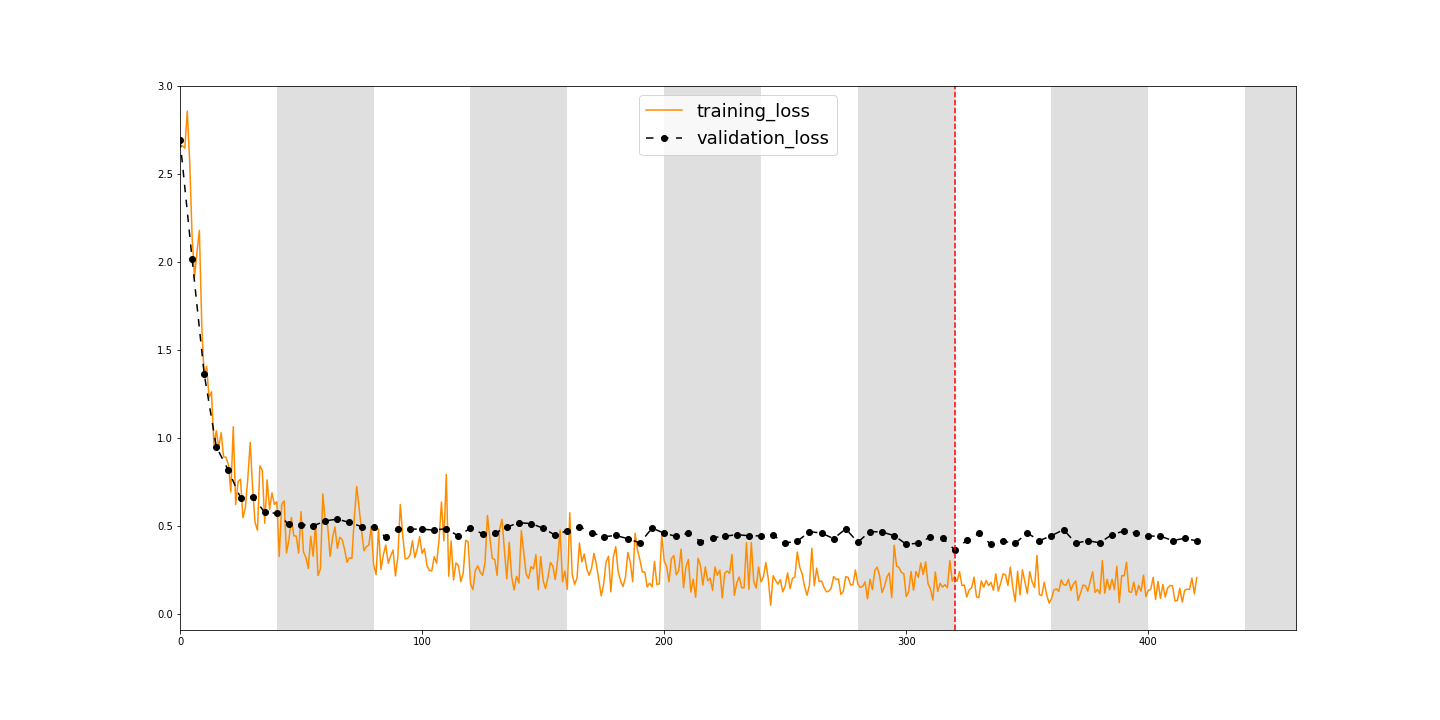
\includegraphics[width=.49\textwidth]{img/loss_finetune.png}}
	{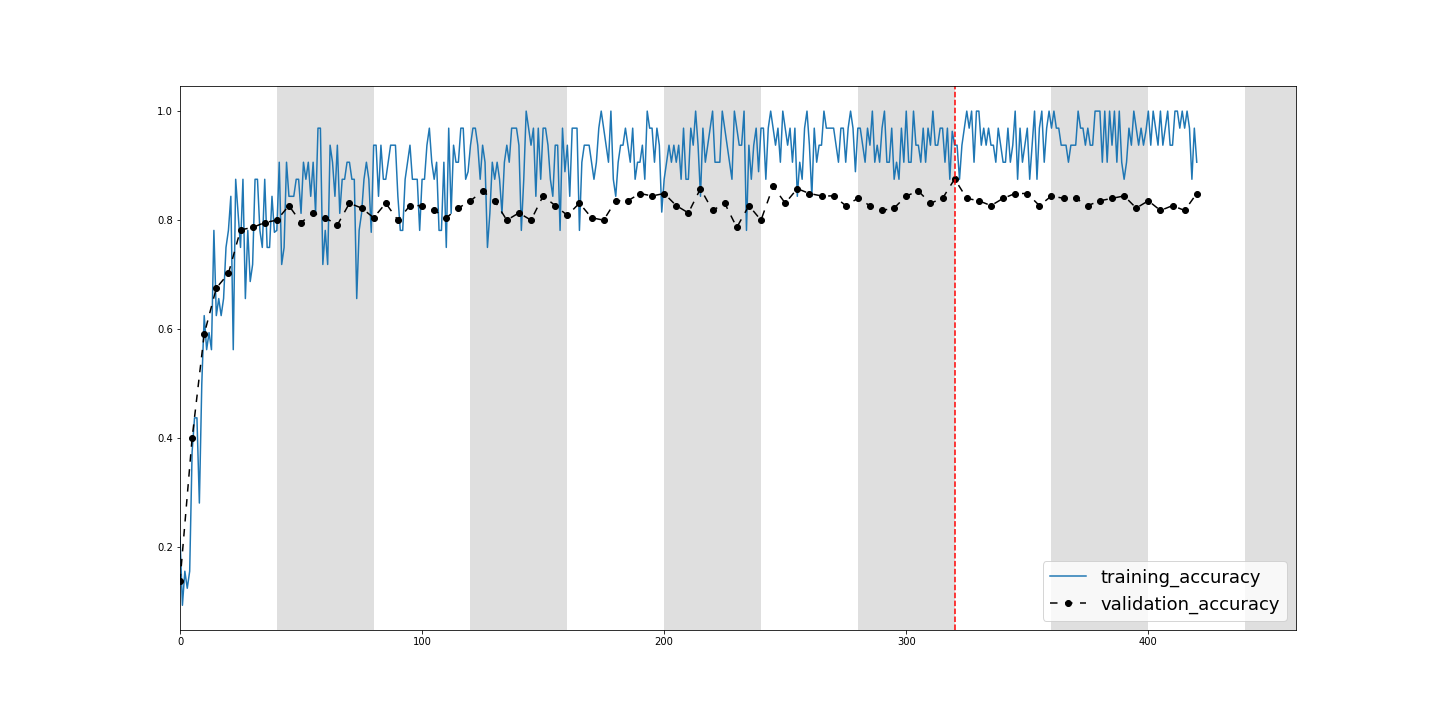
\includegraphics[width=.49\textwidth]{img/acc_finetune.png}}
	\caption{Training and validation accuracy and loss of the finetuned Alexnet}
	\label{fig:finetune}
\end{figure}

The training stops after about 8-10 epochs where we get validation loss around 0.36 and validation accuracy around 0.87. 
Looking at these plots I can see that, as expected, training loss goes to zero while validation loss reaches a plateau and it starts to slightly increase, so we stop the training.
A similar consideration can be done for the accuracy: the training one goes to 1 while the validation one stops increasing after some epochs.

Since the majority of the layers are  pretrained, they weights are already optimized to extract features from images and categorize them. Hence we need just a few iterations to tune the last layer's weights. Indeed the loss rapidly decreases and the accuracy rapidly increases

We can now evaluate the network on the test images and we get a test accuracy of about 0.86:

\begin{center}
	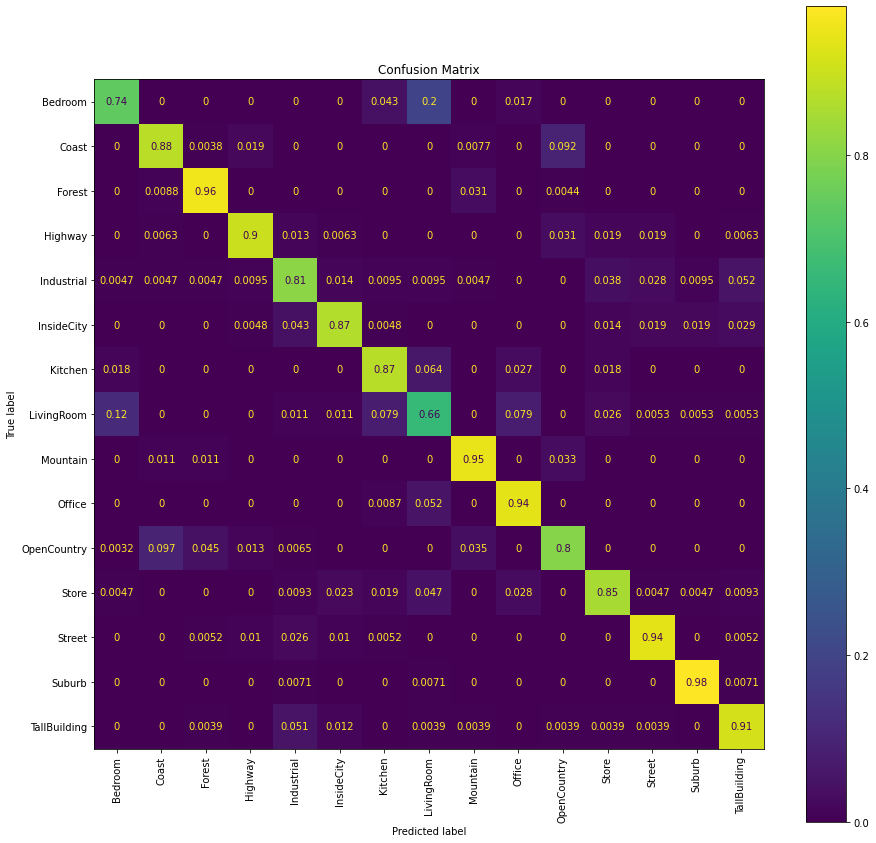
\includegraphics[width=\textwidth]{img/conf_finetune.png}	
\end{center}
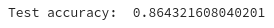
\includegraphics[width=0.3\textwidth]{img/test_accuracy_finetune.png}

The majority of the test images are correctly classified, but we still have some misclassifications.
It's interesting to see that some images are misclassified in classes which are kind of similar, for example I have some misclassifications between house rooms (bedroom-living room-kitchen) and between natural scenes (coast-forest-open country).

\subsection*{3.2 CNN as feature extractor + SVM}

\subsubsection*{Problem statement}
Use a pretrained convolutional neural network to extract features from an image and then train a multiclass classifier based on support vector machines.

\subsubsection*{Approach}
The feature vector is extracted accessing the activations of an intermediate layer of the pretrained neural network.
The multiclass classification problem is faced using pairwise linear svm with decision tree. 
First we learn a classifier for each pair of classes, then each node of the decision tree will perform the classification of an image using one of the trained binary classifiers. 
The classification will then continue on the left or right subtree where the 'losing' class is excluded. We proceed in this way until we are left with only two possible classes, the predicted class is the output of this last classifier.

\subsubsection*{Implementation choices}
We use again Alexnet to extract a vector of features from each image. In particular we use just the 'feature' layers of the net, here the architecture

\begin{table}[h!]
	\centering
	\begin{tabular}{lll}
		\# & Type & Size \\
		\midrule
		Features & & \\
		1 & Image Input & 224x224x3 images \\
		2 & Convolution & 64 11x11 convolutions with stride 4 \\
		3 & ReLu & \\
		4 & Max Pooling & 3x3 max pooling with stride 2 \\
		5 & Convolution & 192 5x5 convolutions with stride 1 \\
		6 & ReLu & \\
		7 & Max Pooling & 3x3 max pooling with stride 2 \\
		8 & Convolution & 384 3x3 convolutions with stride 1 \\
		9 & ReLu & \\
		10 & Convolution & 256 3x3 convolutions with stride 1 \\
		11 & ReLu & \\
		12 & Max Pooling & 3x3 max pooling with stride 2 \\
		\bottomrule
		\label{tab:baseline}
	\end{tabular}
\end{table}

We will get feature vectors of length 9216 which are used to train a multiclass support vector machine classifier. 	
First let's discuss the construction of the decision tree, then we will focus on how to train each binary classifiers.

\begin{description}
	\item[\textbf{Decision tree:}] 
	Each node of the tree will contain the 2 classes to be compared, the function to perform the comparison and 2 pointers to other nodes which will be the left child and right child.
	It's a good idea to put in the higher part of the tree classes which are easily separable. In order to do so, when we train all the binary classifiers we will also store the number of support vectors, a measure of the generalization capability of the model.
	
	In this way we can start building the tree from the root in a recursive way: we use a specific function that given the list of classes selects the most separable two, builds the node and sets as right and left children two nodes built in the same way but operating on the sublists in which one of the two selected classes is removed.
	The recursive calls terminate when we have to build a node from a list with just two classes. In this case the node will not have any children.
	
	Once the tree is built I need a way to perform a binary classification on each node. In this way an image can go through the tree and be classified.
	In order to do this each node has an evaluate function which, given the image and the two classes, accesses the correspondent binary classifier and decides if to send the image to the left child or to the right child. In the new node it will be evaluated again in the same way until a leaf is reached and we will get the predicted class. 
	
	I cannot process a batch of testing images all together because each image will follow a different path and go through 14 classifiers regardless the path.
	This causes the testing phase to significantly slow down.
	
	The evaluation in each node corresponds to the decision function of a binary classifier. Hence now we need to discuss how to build each svm classifier and the correspondent decision function.
	
	
	\item[\textbf{Pairwise svm:}] Since we need to manage images of just two classes we don't use the training dataloaders as in section 1 but we load the whole dataset (relatively small), accessing then just the needed images for each classifier. In this way we can avoid to load many times the same images in memory.
	
	The training of the svm classifier consist in solving the following quadratic programming problem (dual formulation):
	$$
	\min_{\alpha}\quad \sum_{i=1}^{l}\alpha_i - \frac{1}{2}\sum_{i,j} \alpha_i \alpha_j y_i y_jk(x_i,x_j)
	$$ 
	$$
	s.t. \quad \sum_{i=1}^{l} \alpha_i y_i = 0; \qquad
	0\leq \alpha_i \leq C, \forall i=1,...,l
	$$
	
	Thanks to the library cvxopt, setting the parameter C equal to 1 and deciding which kernel to use we are able to solve this optimization and to find the vector $\alpha$.
	In the first place we work with the linear kernel and we can identify the support vectors as the ones having $alpha$ significantly different from 0 ($\geq 1e-6$).
	The threshold has been chosen empirically looking at the vector $\alpha$ and we use the linear kernel $k(x_i,x_j)= <x_,x_j>$.
	
	
	For each optimization we store in a matrix the support vectors $X^*$ and the correspondent labels $y^*$ and $\alpha^*$.
	Moreover we store the number of support vectors to build the decision tree as described above.
	
	Now we can build the decision function for a new image $x$:
	$$
	h(x) = \Theta(\sum_{SV} y_i\alpha_i k(x_i,x) + b)
	$$
	
	where $b$ can be computed from any unbounded support vector in the following way:
	
	$$
	b = y_i - \sum_{SV} y_j\alpha_ik(x_j,x_i)
	$$
	
	To avoid bounded support vectors having $\alpha_i \simeq C$ we first chose to use the support vector having the minimum value $\alpha_i$. But in this way the decision function was not working for some pair of classes (maybe numerical problems because $\alpha_i$ very close to 0). We fixed the problem computing $b_i$ for any support vector and then using the average value.
	
\end{description}

Now we are able to train all the pairwise svm, build the decision tree and evaluate the classifier on the test set.



\subsubsection*{Results}
Using the classifier with the linear kernel gives us a test accuracy of about 87\%:

\begin{center}
	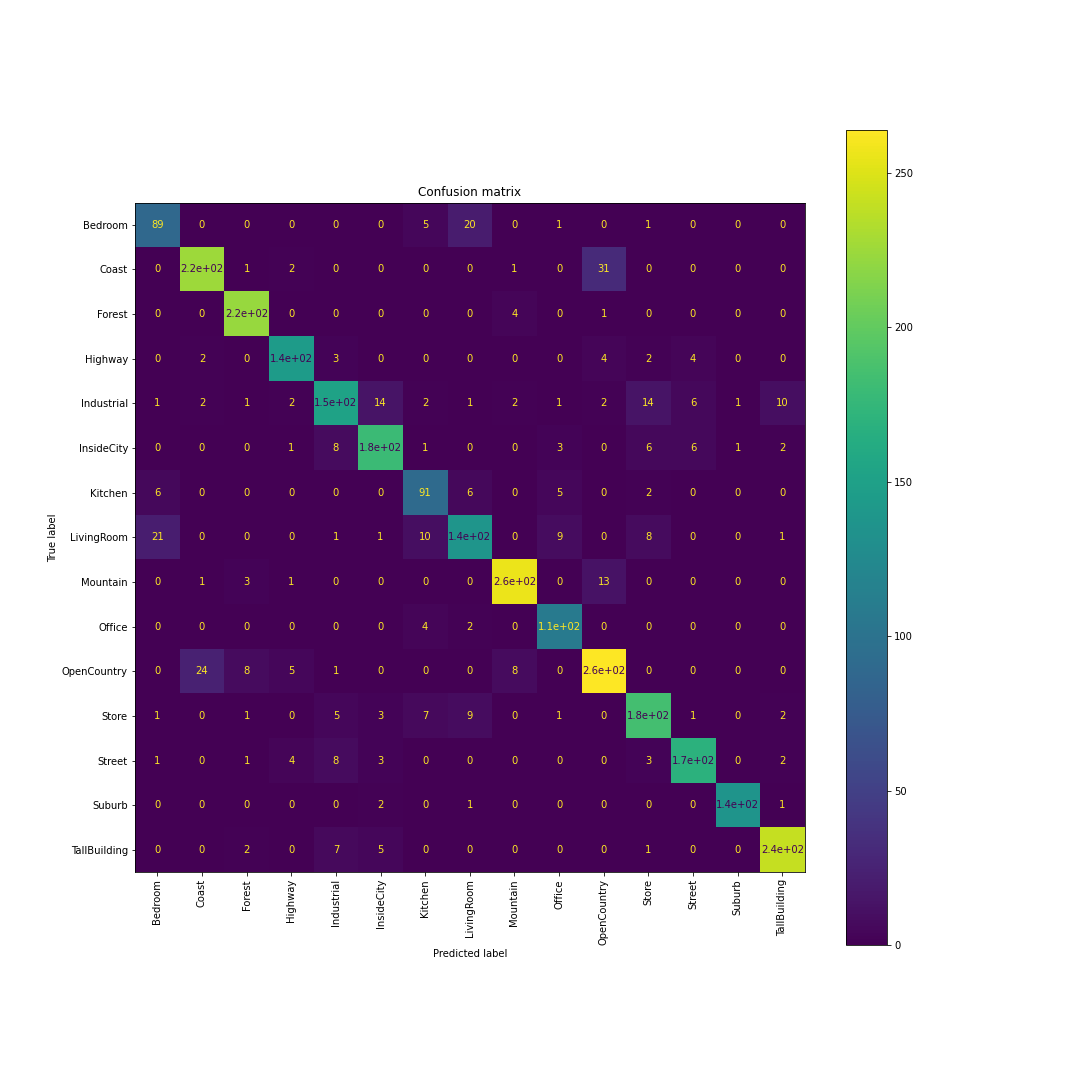
\includegraphics[width=\textwidth]{img/confusion_multiclassSVM.png}	
\end{center}
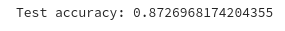
\includegraphics[width=0.3\textwidth]{img/test_accuracy_multiSVM.png}

The confusion matrix is very similar to the one obtained finetuning Alexnet, also the classes which are misclassified the most are the same.

\begin{thebibliography}{9}
	
	\bibitem{Lazebnik et al., 2006}
	Lazebnik, S., Schmid, C., and Ponce, J.
	\textit{Beyond bags of features: Spatial pyramid matching for recognizing natural scene
	categories}
	In 2006 IEEE Computer Society Conference on Computer Vision	and Pattern Recognition (CVPR’06), volume 2, pages 2169–2178.
	
	\bibitem{Ioffe and Szegedy, 2015}
	Ioffe, S. and Szegedy, C.
	\textit{Batch normalization: Accelerating deep network training by reducing internal covariate shift}
	2015, arXiv	preprint arXiv:1502.03167
	
	\bibitem{Szegedy et al., 2015}
	\textit{Going deeper with convolutions}
	Szegedy, C., Liu, W., Jia, Y., Sermanet, P., Reed, S., Anguelov, D., Erhan, D., Vanhoucke, V., and Rabinovich, A. (2015). In The IEEE Conference on Computer Vision and Pattern Recognition (CVPR).
	
\end{thebibliography}


\end{document}

